\chapter{Zintuiglijke stelsels}\label{ch:b3:sensory-systems}

In een donkere nacht kan een menselijk oog een flits van enkele fotonen
waarnemen --- de kleinste hoeveelheid licht die de natuurkunde
überhaupt toelaat waar te nemen. Het oor hoort een geluid dat het
trommelvlies over minder dan de diameter van een waterstofatoom
beweegt, en onderscheidt een toon van een andere die er een vijfde
procent van verschilt. Een hond volgt een spoor van enkele moleculen
per kubieke centimeter; een haai vindt een schol onder het zand aan het
elektrische veld van haar hartslag. Elk zintuig begint met een cel die
één soort energie omzet in een verandering van de membraanpotentiaal,
en elk zintuig eindigt als pulsen in een zenuw; daartussen liggen de
vraagstukken die dit hoofdstuk behandelt: hoe een receptor één enkel
molecuul of foton versterkt tot een signaal dat een neuron kan lezen,
hoe een biljoenvoudig bereik aan sterkte wordt geperst in een tempo van
enkele honderden pulsen per seconde, hoe een mechanische golf naar
frequentie wordt gesorteerd, hoe tienduizend geuren met vierhonderd
receptoren uit elkaar worden gehouden, en hoe het brein, dat nooit iets
anders dan pulsen ontvangt, weet van welk zintuig zij komen.

\section{Beginselen die elk zintuig deelt}

\begin{definition}[Omzetting, codering en aanpassing]\label{def:b3:sensory-systems:principles}
\index{zintuiglijke omzetting}\index{receptorpotentiaal}\index{gemerkte lijn}\index{receptief veld}\index{aanpassing!zintuiglijk}\index{laterale remming}
Een \emph{zintuiglijke receptorcel} bevat een
\emph{omzettingsmechanisme} --- een eiwit of een cascade --- dat een
prikkel (een foton, een molecuul, een verplaatsing, warmte, een
elektrisch veld) omzet in een verandering van de membraangeleiding en
daarmee in een \emph{receptorpotentiaal}, die met de prikkel meeloopt;
de cel, of het neuron waarop zij overschakelt, maakt daarvan een reeks
actiepotentialen wier tempo de sterkte codeert. De \emph{modaliteit}
van een signaal wordt niet gegeven door de pulsen, die in elke zenuw
gelijk zijn, maar door de draad waarlangs zij reizen en door waar die
in het brein eindigt: een \emph{gemerkte lijn}. Een zintuiglijk neuron
antwoordt op prikkels binnen een \emph{receptief veld} --- een stukje
huid, een gebied van het gezichtsveld, een band van frequenties --- en
naburige velden scherpen elkaar door \emph{laterale remming}, waarbij
elk neuron zijn buren onderdrukt zodat randen en contrasten worden
overdreven. De meeste receptoren \emph{passen zich aan}: hun antwoord
op een aanhoudende prikkel neemt af, zodat zij verandering melden in
plaats van niveau, en hun werkbereik verschuift naar de heersende
achtergrond.
\end{definition}

\begin{theorem}[Weber, Fechner en Stevens]\label{thm:b3:sensory-systems:weber}
\index{wet van Weber}\index{wet van Fechner}\index{machtswet van Stevens}
De waarneming van Weber (1834) is dat de kleinste merkbare verandering
$\Delta I$ in een prikkel van sterkte $I$ een vast deel daarvan is:
$\Delta I/I = k$, met $k$ ongeveer $0.02$ voor gewicht, $0.08$ voor
helderheid, $0.1$ voor luidheid. Telt men elk net merkbaar verschil als
één eenheid van gewaarwording $S$, dan is $\mathrm{d}S = \mathrm{d}I/
(kI)$ en
\[
S = \frac{1}{k}\ln\frac{I}{I_{0}} ,
\]
waarin $I_{0}$ de drempel is: de gewaarwording groeit als de logaritme
van de prikkel (Fechner, 1860), en daarom worden sterkten in \omterm{def:b3:sensory-systems:cochlea}{decibel} en
magnituden gemeten, en daarom valt een kaars die bij een kaars wordt
gezet op en een kaars die bij een schijnwerper wordt gezet niet.
Rechtstreekse schaalproeven, waarin proefpersonen getallen aan
gewaarwordingen toekennen, geven in plaats daarvan een machtswet
$S \propto I^{n}$ (Stevens, 1957), met $n \approx
0.3$ voor luidheid en helderheid, $1$ voor lijnlengte en $3.5$ voor
elektrische schokken; een logaritme en een kleine macht zijn over
enkele decaden nauwelijks te onderscheiden, en beide wetten zijn het
eens over het wezenlijke: het zenuwstelsel comprimeert.
\end{theorem}
\begin{proof}
Uit $\Delta I = kI$ voor één eenheid van $S$ volgt dat de toename van
de gewaarwording per toename van de prikkel $\mathrm{d}S/\mathrm{d}I = 1/(kI)$ is;
integratie vanaf de drempel $I_{0}$, waar $S = 0$, geeft $S = (1/k)
\ln(I/I_{0})$. De machtswet is de andere aanname, dat een vaste
\emph{verhouding} van prikkels een vaste \emph{verhouding} van
gewaarwordingen oplevert,
$\mathrm{d}S/S = n\,\mathrm{d}I/I$, waarvan de integraal $S \propto I^{n}$ is;
voor $n \to 0$ nadert zij bij geschikte schaling de logaritme.
\end{proof}

\begin{omfigure}
\begin{tikzpicture}
\begin{axis}[
  width=0.68\linewidth, height=5.6cm,
  xmode=log,
  xmin=1, xmax=1e6, ymin=0, ymax=15,
  xlabel={prikkelsterkte $I/I_{0}$}, ylabel={gewaarwording $S$ (willekeurig)},
  xlabel style={font=\small, at={(axis description cs:0.5,-0.12)}, anchor=north}, ylabel style={font=\small},
  tick label style={font=\small}, ytick={0,5,10,15},
  clip=false,
]
\addplot[very thick, omDef, domain=1:1e6, samples=100] {ln(x)};
\addplot[very thick, omThm, domain=1:1e6, samples=100] {0.235*x^0.3 - 0.235};
\addplot[very thick, omMeth!70!black, domain=1:1e6, samples=100] {0.5*x^0.24 - 0.5};
\node[font=\scriptsize, omDef, anchor=north west] at (axis cs:2,10.2) {Fechner: $S = \ln(I/I_{0})$};
\node[font=\scriptsize, omThm, anchor=south east] at (axis cs:9e5,0.4) {Stevens: $S \propto I^{0.3}$};
\node[font=\scriptsize, omMeth!70!black, anchor=north west] at (axis cs:2,12.5) {Stevens: $S \propto I^{0.24}$};
\end{axis}
\end{tikzpicture}

{\small Compressie van een miljoenvoudig bereik aan sterkte tot een
gewaarwording die traag groeit: de logaritme van Fechner en de
machtswetten van Stevens met kleine exponenten zijn over enkele decaden
moeilijk uit elkaar te houden, en beide zeggen dat de zintuigen
verhoudingen melden, geen verschillen.}
\end{omfigure}

\section{Het zien}

\begin{definition}[Het netvlies]\label{def:b3:sensory-systems:retina}
\index{netvlies}\index{staafje}\index{kegeltje}\index{fototransductie}\index{rodopsine}\index{ganglioncel}\index{centrum--omgeving}
Het \emph{netvlies} is een blad brein achter in het oog, drie lagen
cellen met de fotoreceptoren, paradoxaal genoeg, achteraan, tegen het
pigmentepitheel. \emph{Staafjes} --- $10^{8}$ per oog, één pigment,
\emph{rodopsine} --- dienen het schemerlicht en raken in daglicht
verzadigd; \emph{kegeltjes} --- $6\times 10^{6}$, drie pigmenten met
pieken in het blauw, het groen en het rood, opeengepakt in de fovea ---
dienen het daglicht, de kleur en de scherpte. \emph{Fototransductie} is
een cascade: een foton isomeriseert de retinale chromofoor van één
rodopsine; het geactiveerde rodopsine zet honderden moleculen van het
G-eiwit transducine aan, die elk een fosfodi-esterase activeren dat
cyclisch GMP afbreekt; de daling van cGMP sluit de kationkanalen die
het cGMP in het donker openhield, de inwaartse ``donkerstroom'' stopt,
en de cel \emph{hyperpolariseert} --- licht zet een fotoreceptor uit,
en zij geeft minder glutamaat af. In het donker is de cel
gedepolariseerd en geeft zij onophoudelijk af. Het signaal gaat door
naar \emph{bipolaire cellen} (van het ON- en het OFF-type, die het
omkeren of behouden) en verder naar de \emph{ganglioncellen}, een
miljoen per oog, wier axonen de oogzenuw vormen --- een honderdvoudige
compressie. Horizontale cellen en amacriene cellen verbinden zijdelings,
en hun remming geeft elke ganglioncel een \omterm{def:b3:sensory-systems:principles}{receptief veld} van het type
\emph{centrum--omgeving}: geprikkeld door licht in een centrale schijf
en geremd door licht in de ring eromheen (of omgekeerd), zodat het
netvlies plaatselijk contrast en randen meldt in plaats van de absolute
hoeveelheid licht.
\end{definition}

\begin{omfigure}
\begin{tikzpicture}[every node/.style={font=\scriptsize}, >=stealth]
  % cascade boxes with amplification numbers
  \node[draw, thick, rounded corners, fill=omProp!30, align=center] (ph) at (0,0) {1 foton};
  \node[draw, thick, rounded corners, fill=omDef!20, align=center] (rh) at (2.6,0) {1 rodopsine*\\(metarodopsine II)};
  \node[draw, thick, rounded corners, fill=omDef!20, align=center] (tr) at (5.6,0) {$\sim 500$ transducines\\geactiveerd};
  \node[draw, thick, rounded corners, fill=omDef!20, align=center] (pde) at (8.6,0) {$\sim 500$ PDE actief:\\$\sim 10^{5}$ cGMP gehydrolyseerd};
  \node[draw, thick, rounded corners, fill=omThm!20, align=center] (ch) at (5.6,-2.0) {$\sim 200$ kationkanalen sluiten;\\donkerstroom daalt met \qty{1}{pA}};
  \node[draw, thick, rounded corners, fill=omMeth!25, align=center] (out) at (1.4,-2.0) {hyperpolarisatie van \qty{1}{mV};\\minder glutamaat afgegeven};
  \draw[->, thick] (ph) -- (rh); \draw[->, thick] (rh) -- (tr); \draw[->, thick] (tr) -- (pde);
  \draw[->, thick] (pde.south) |- (ch.east); \draw[->, thick] (ch) -- (out);
  \node[below, font=\tiny, align=center] at (7.1,-2.8) {elke stap vermenigvuldigt; de hele cascade wordt binnen \qty{200}{ms} afgezet door\\rodopsinekinase, arrestine en het GTPase van transducine, en daarna hersteld};
\end{tikzpicture}

{\small \omterm{def:b3:sensory-systems:retina}{Fototransductie} als versterker. Eén opgenomen foton sluit
honderden kanalen via twee katalytische trappen, een winst van ongeveer
een miljoen in moleculen --- genoeg om met één foton een meetbare
stroom in een \omterm{def:b3:sensory-systems:retina}{staafje} op te wekken.}
\end{omfigure}

\begin{theorem}[Fotonen tellen: de frequentie van het zien]\label{thm:b3:sensory-systems:hecht}
\index{waarneming van één foton}\index{frequentie-van-zien-kromme}\index{Poisson!fotonen tellen}
Een flits die gemiddeld $a$ opgenomen fotonen aan een plek \omterm{def:b3:sensory-systems:retina}{staafjes}
levert, levert bij elke afzonderlijke aanbieding een aantal $k$ dat
Poisson-verdeeld is: $P(k) = e^{-a}a^{k}/k!$. Meldt de waarnemer de
flits te zien zodra er ten minste $n$ fotonen worden opgenomen, dan is
de kans op zien
\[
P_{\text{see}}(a) = 1 - \sum_{k=0}^{n-1} e^{-a}\,\frac{a^{k}}{k!} ,
\]
een kromme die van $0$ naar $1$ stijgt naarmate $a$ toeneemt, en wier
\emph{steilheid} op een logaritmische schaal van $a$ alleen van $n$
afhangt: hoe hoger het drempelaantal, hoe steiler de kromme. Het fitten
van de gemeten \omterm{thm:b3:sensory-systems:hecht}{frequentie-van-zien-kromme} geeft dus $n$ zonder dat
bekend hoeft te zijn hoeveel van de geleverde fotonen werkelijk zijn
opgenomen.
\end{theorem}
\begin{proof}
Fotonen uit een zwakke, gelijkmatige bron komen onafhankelijk en
willekeurig aan, en het aantal dat in een korte flits uit een
gemiddelde $a$ wordt opgenomen is Poisson-verdeeld (de limiet van een
binomiale verdeling met veel fotonen die elk met kleine kans worden
opgenomen). Zien vergt $k \ge n$, waarvan de kans één min de som van de
eerste $n$ Poisson-termen is. De bron met een factor $c$ schalen
vermenigvuldigt $a$ met $c$ en verschuift de kromme langs de as van $\log a$
zonder haar vorm te veranderen, dus wijst de vorm $n$ aan: voor $n =
1$ stijgt $P = 1 - e^{-a}$ over twee decaden van $a$; voor $n = 6$
stijgt zij over minder dan één.
\end{proof}

\begin{proof}[Bewijsmateriaal]
Hecht, Shlaer en Pirenne (1942) lieten waarnemers een half uur in het
donker zitten en flitsten daarna gedurende een milliseconde een
piepklein groen stipje op de staafjesrijke rand van het \omterm{def:b3:sensory-systems:retina}{netvlies},
honderden malen bij verschillende sterkten, en noteerden het aandeel
geziene flitsen. De drempelflits bevatte aan het hoornvlies zo'n $90$
fotonen, waarvan er (na weerkaatsing, opname in de media van het oog en
de kans van $20\,\%$ dat een foton dat een \omterm{def:b3:sensory-systems:retina}{staafje} bereikt door
\omterm{def:b3:sensory-systems:retina}{rodopsine} wordt opgenomen) ongeveer $5$--$14$ werden opgenomen. De
\omterm{thm:b3:sensory-systems:hecht}{frequentie-van-zien-krommen} hadden de steilheid van
$n = 5$ tot $7$: de waarnemer zei ``ja'' wanneer ongeveer zes \omterm{def:b3:sensory-systems:retina}{staafjes},
van de vijfhonderd onder het stipje, elk één foton hadden opgevangen.
Eén \omterm{def:b3:sensory-systems:retina}{staafje} neemt één foton waar; het brein eist er enkele tegelijk, om
de valse meldingen uit de spontane isomerisaties van de \omterm{def:b3:sensory-systems:retina}{staafjes} ---
één per \omterm{def:b3:sensory-systems:retina}{staafje} per veertig seconden --- onder het tempo van de sterren
te houden.
\end{proof}

\begin{omfigure}
\begin{tikzpicture}
\begin{axis}[
  width=0.68\linewidth, height=5.6cm,
  xmode=log,
  xmin=0.1, xmax=100, ymin=0, ymax=1.05,
  xlabel={gemiddeld opgenomen fotonen per flits, $a$}, ylabel={kans op zien},
  xlabel style={font=\small, at={(axis description cs:0.5,-0.12)}, anchor=north}, ylabel style={font=\small},
  tick label style={font=\small}, ytick={0,0.5,1},
  clip=false,
]
\addplot[very thick, omDef, domain=0.1:100, samples=120] {1-exp(-x)};
\addplot[very thick, omProp, domain=0.1:100, samples=120] {1-exp(-x)*(1+x+x^2/2)};
\addplot[very thick, omThm, domain=0.1:100, samples=120] {1-exp(-x)*(1+x+x^2/2+x^3/6+x^4/24+x^5/120)};
\node[font=\scriptsize, omDef, anchor=north west] at (axis cs:0.12,0.95) {$n = 1$};
\node[font=\scriptsize, omProp, anchor=north west] at (axis cs:1.1,0.5) {$n = 3$};
\node[font=\scriptsize, omThm, anchor=north west] at (axis cs:5.5,0.45) {$n = 6$};
\end{axis}
\end{tikzpicture}

{\small \omterm{thm:b3:sensory-systems:hecht}{Frequentie-van-zien-krommen} voor drempels van één, drie en zes
opgenomen fotonen. Hoe steiler de kromme, hoe meer fotonen moeten
samenvallen; de waarnemers van Hecht gaven krommen als de rode.}
\end{omfigure}

\begin{omfigure}
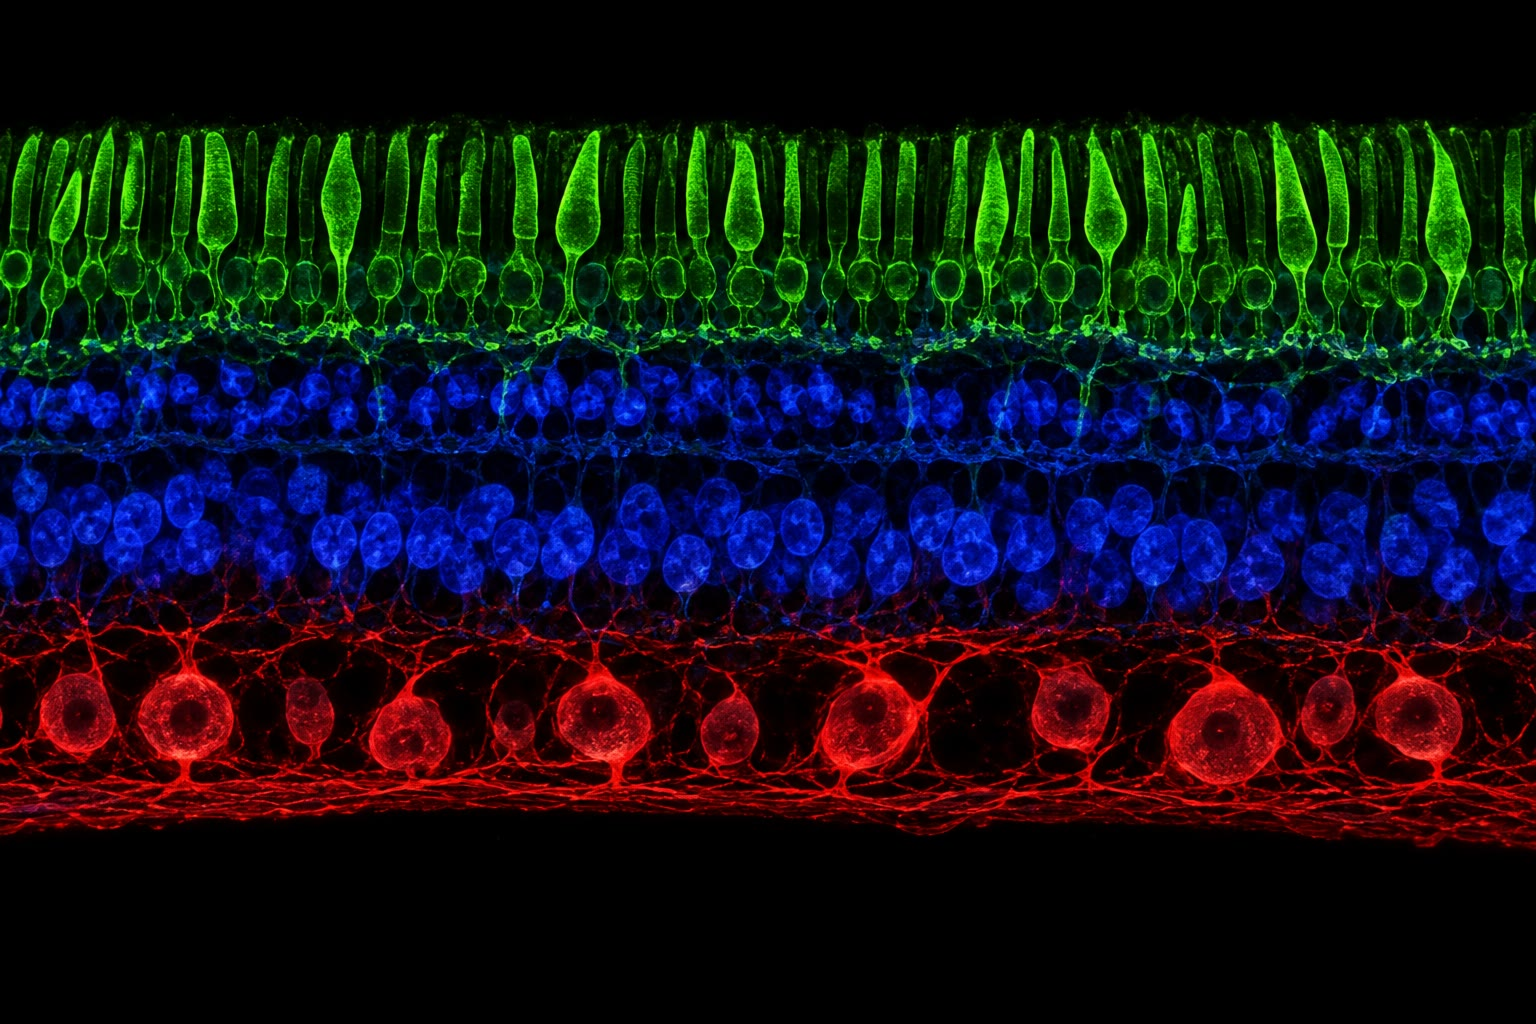
\includegraphics[width=0.46\linewidth]{images/book5/ai/b5-18-retina-section.jpg}\hspace{0.04\linewidth}
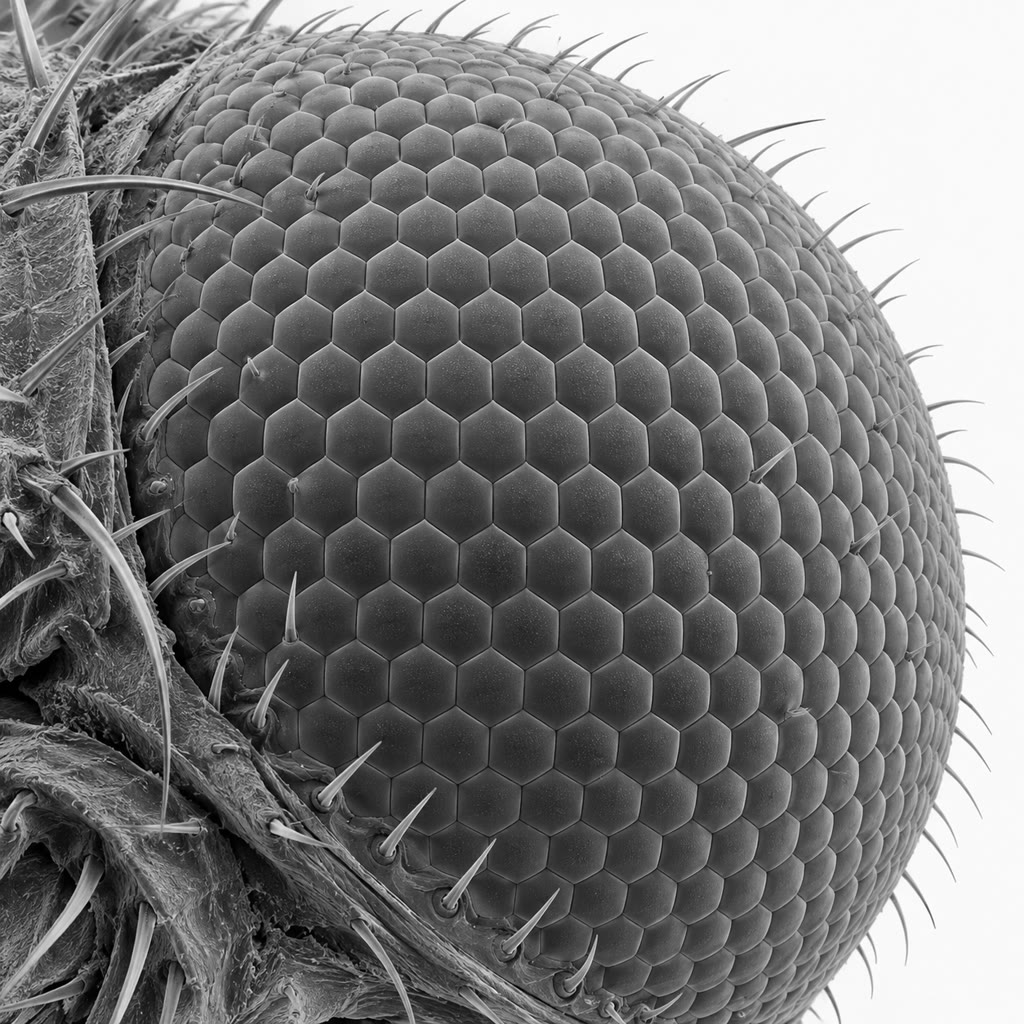
\includegraphics[width=0.36\linewidth]{images/book5/ai/b5-18-compound-eye.jpg}

{\small Links: een doorsnede van het \omterm{def:b3:sensory-systems:retina}{netvlies}, met de fotoreceptoren
(groen) achteraan, dan de bipolaire cellen en de horizontale cellen,
dan de ganglioncellen (rood) wier axonen naar het brein vertrekken.
Rechts: het samengestelde oog van een vlieg, honderden afzonderlijke
lenzen die elk hun eigen receptoren hebben --- een andere oplossing voor
hetzelfde probleem.}
\end{omfigure}

\section{Gehoor en evenwicht}

\begin{definition}[Het slakkenhuis]\label{def:b3:sensory-systems:cochlea}
\index{slakkenhuis}\index{basilair membraan}\index{tonotopie}\index{haarcel}\index{stereocilia}\index{tipverbinding}\index{decibel}
Geluid is een drukgolf; het probleem van het oor is drukveranderingen
van enkele tientallen micropascal in lucht waar te nemen en ze naar
frequentie te sorteren. Het trommelvlies en de drie gehoorbeentjes van
het middenoor bundelen de kracht van de \qty{55}{mm^2} van het vlies op
de \qty{3}{mm^2} van het ovale venster, wat de druk zo'n twintigvoudig
verhoogt --- de impedantie-aanpassing tussen lucht en de vloeistof van
het binnenoor, zonder welke het meeste geluid zou weerkaatsen. In het
\emph{slakkenhuis}, een opgerolde buis van \qty{35}{mm}, loopt de
drukgolf langs het \emph{basilaire membraan}, dat aan de basis smal en
stijf is en aan de top breed en slap; elke frequentie laat het membraan
het sterkst op één plaats trillen --- hoge frequenties nabij de basis,
lage nabij de top --- een \emph{tonotopische} kaart die het brein als
toonhoogte leest. Op het membraan zitten de \emph{haarcellen}:
\num{3500} binnenste haarcellen op één rij, elk bekroond met een bundel
\emph{stereocilia} die punt aan punt door fijne
\emph{tipverbindingen} zijn verbonden; de bundel naar zijn langste
cilium buigen rekt de verbindingen en trekt binnen microseconden
kationkanalen open, zonder enige tweede boodschapper, en kalium stroomt
naar binnen vanuit de endolymfe, wier ongewone samenstelling en
potentiaal van $+\qty{80}{mV}$ een drijvende kracht van \qty{150}{mV}
geven. De binnenste haarcellen melden aan de gehoorzenuw; de
\num{12000} buitenste haarcellen, door dezelfde beweging aangedreven,
trekken samen en rekken uit met het geluid door het motoreiwit prestine
en pompen energie terug in de trilling van het membraan --- een
versterker die de afstemming honderdvoudig scherpt en die bij de meeste
doofheid uitvalt. De sterkte wordt in \emph{decibel} gemeten: $L = 10\log_{10}
(I/I_{0})$, met $I_{0} = \qty{1e-12}{W/m^2}$ de gehoordrempel; het oor
werkt over \qty{120}{dB}, een biljoenvoud in sterkte.
\end{definition}

\begin{omfigure}
\begin{tikzpicture}[every node/.style={font=\scriptsize}, >=stealth]
  % unrolled cochlea
  \begin{scope}
    \draw[thick, omDef, fill=omDef!10] (0,0.9) -- (7,1.4) -- (7,-1.4) -- (0,-0.9) -- cycle;
    \draw[very thick, omProp] (0,0.15) -- (7,-0.15); \draw[very thick, omProp] (0,-0.15) -- (7,0.15);
    \node[above] at (0.8,1.05) {basis: smal, stijf}; \node[above] at (6.2,1.5) {top: breed, slap};
    \node[left, align=right] at (-0.1,0) {ovale venster\\(vanaf de\\stijgbeugel)};
    \foreach \x/\f in {0.9/\qty{16}{kHz}, 2.3/\qty{4}{kHz}, 3.8/\qty{1}{kHz}, 5.4/\qty{250}{Hz}, 6.6/\qty{60}{Hz}} { \draw[omThm, thick] (\x,-0.55) -- (\x,0.55); \node[below, omThm] at (\x,-0.65) {\f}; }
    \node[below, align=center] at (3.5,-1.7) {basilair membraan (oranje): elke frequentie\\trilt het sterkst op één plaats --- tonotopie};
  \end{scope}
  % hair cell mechanism
  \begin{scope}[xshift=8.2cm, yshift=-0.6cm]
    \draw[thick, fill=omMeth!20] (0,0) rectangle (1.6,1.2); \node[below] at (0.8,-0.05) {haarcel};
    \foreach \x/\h in {0.35/0.6, 0.65/0.85, 0.95/1.1, 1.25/1.35} \draw[very thick, omMeth!70!black] (\x,1.2) -- (\x,1.2+\h);
    \foreach \x/\h/\xx/\hh in {0.35/0.6/0.65/0.85, 0.65/0.85/0.95/1.1, 0.95/1.1/1.25/1.35} \draw[omThm, thick] (\x,1.2+\h) -- (\xx,1.2+\hh-0.1);
    \draw[->, thick] (1.9,2.3) -- (2.4,2.3) node[right, align=left, font=\tiny] {buig naar de langste:\\tipverbindingen rekken,\\kanalen openen in\\$\unit{\micro s}$; K$^{+}$ stroomt\\binnen (\qty{150}{mV}\\drijfkracht)};
    \node[above, align=center] at (0.8,2.7) {stereocilia verbonden\\door tipverbindingen (rood)};
  \end{scope}
\end{tikzpicture}

{\small Links: het \omterm{def:b3:sensory-systems:cochlea}{slakkenhuis} uitgerold --- het \omterm{def:b3:sensory-systems:cochlea}{basilaire membraan}
verloopt van stijf naar slap, en elke frequentie piekt op haar eigen
plaats. Rechts: een haarbundel, wier \omterm{def:b3:sensory-systems:cochlea}{tipverbindingen} de
omzettingskanalen mechanisch openen wanneer de bundel wordt gebogen.}
\end{omfigure}

\begin{proof}[Bewijsmateriaal]
Von Békésy (jaren 1940) opende de slakkenhuizen van lijken, strooide
zilverdeeltjes op het \omterm{def:b3:sensory-systems:cochlea}{basilaire membraan} en zag onder stroboscopisch
licht hoe zuivere tonen een lopende golf opwekten wier piek dichter bij
de basis lag naarmate de toon hoger was --- de plaatscode, waarvoor hij
in 1961 de Nobelprijs kreeg. Hudspeth (jaren 1980) duwde met een
glasvezel tegen één haarbundel en registreerde de stroom: die vloeide
binnen \qty{10}{\micro s} na de duw, veel te snel voor enige
enzymcascade, evenredig met hoe ver de bundel naar zijn langste rij
bewoog, en zij verdween wanneer de \omterm{def:b3:sensory-systems:cochlea}{tipverbindingen} met een
calciumbinder werden doorgeknipt. Het openen is mechanisch --- de
verbinding trekt het kanaal open --- en daarom is het gehoor het
snelste van de zintuigen en daarom wordt zijn omzetter vernield door de
harde geluiden die de verbindingen breken.
\end{proof}

\begin{example}[De getallen van het oor]\label{ex:b3:sensory-systems:ear-numbers}
Aan de gehoordrempel beweegt het \omterm{def:b3:sensory-systems:cochlea}{basilaire membraan} ongeveer
\qty{0.1}{nm} en is de drukamplitude \qty{20}{\micro Pa}, een twee
miljardste van de luchtdruk; bij \qty{120}{dB} is de druk een miljoen
maal groter en is de beweging van het membraan enkele tientallen
nanometer. Een jong oor hoort van \qty{20}{Hz} tot \qty{20}{kHz} en
scheidt tonen die \qty{0.3}{\%} uiteen liggen, waarbij het onderscheid
van de plaatscode door de buitenste \omterm{def:b3:sensory-systems:cochlea}{haarcellen} wordt gescherpt. De
\num{30000} vezels van de gehoorzenuw vuren tot ongeveer \qty{4}{kHz}
in de maat met de drukgolf (fasevergrendeling) en dragen de
tijdsordening met een nauwkeurigheid van tientallen microseconden over,
waaruit het brein de richting van een geluid berekent uit het verschil
in aankomst bij de twee oren --- soms niet meer dan \qty{10}{\micro s}.
De evenwichtsorganen gebruiken dezelfde \omterm{def:b3:sensory-systems:cochlea}{haarcellen}: in de
\emph{halfcirkelvormige kanalen} buigt de traagheid van de vloeistof ze
wanneer het hoofd draait (hoekversnelling), en in de otolietorganen
belast een laagje kristallen van calciumcarbonaat ze met de zwaartekracht
en de lineaire versnelling.
\end{example}

\begin{omfigure}
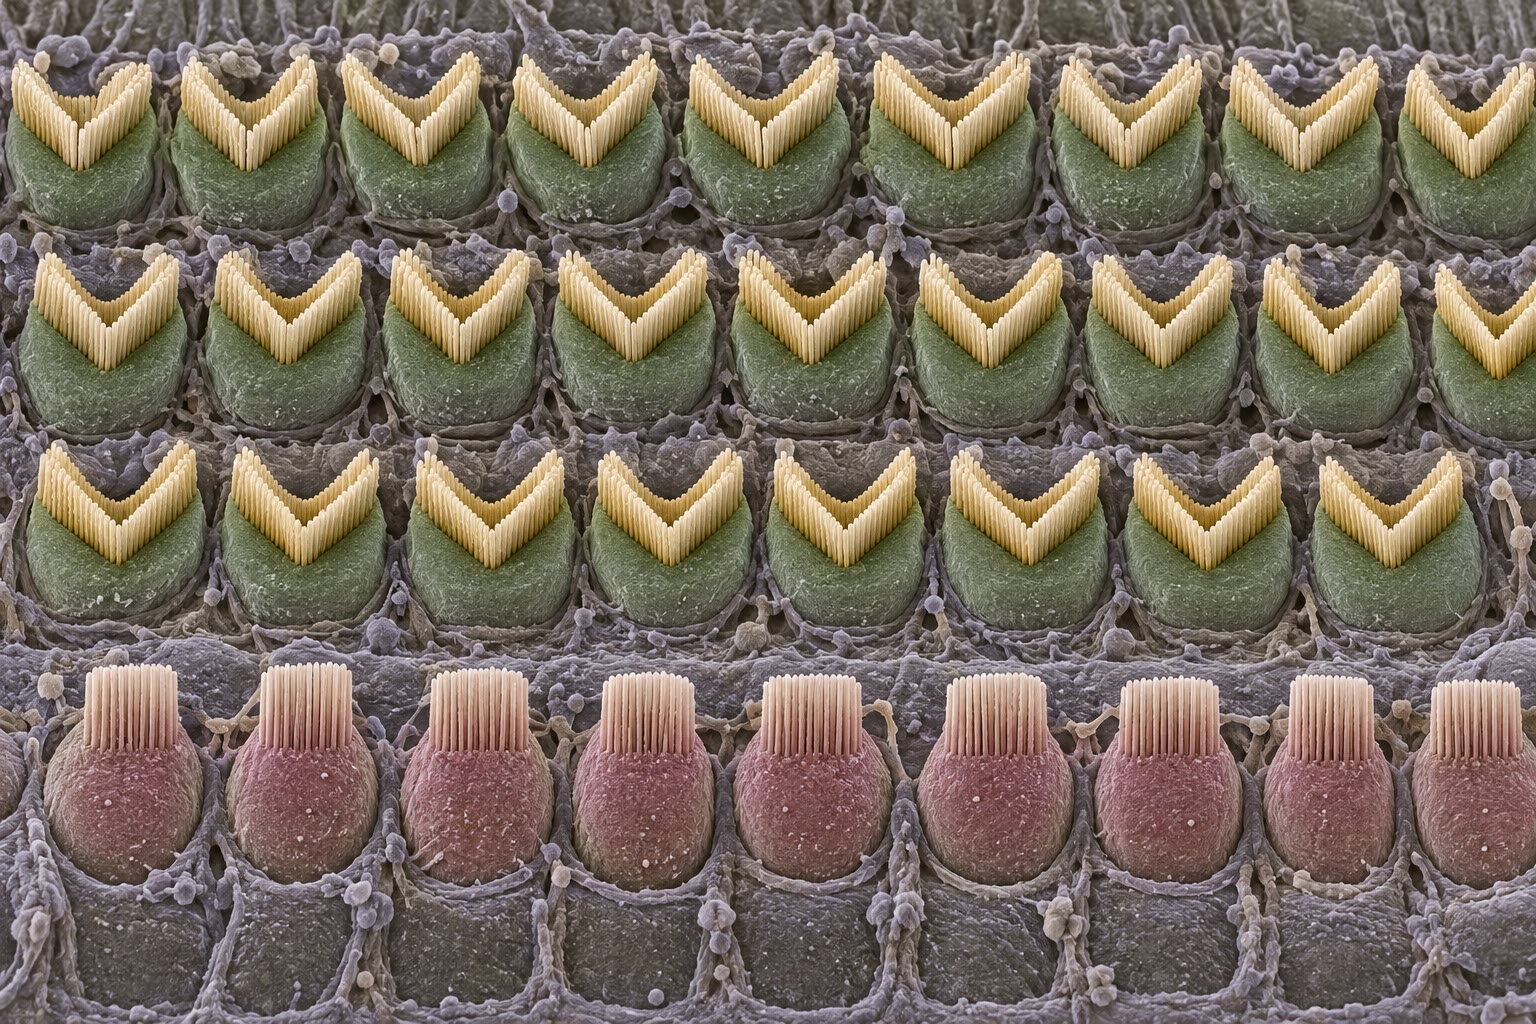
\includegraphics[width=0.54\linewidth]{images/book5/ai/b5-18-cochlea-hair-cells.jpg}

{\small Het orgaan van Corti van bovenaf: drie rijen buitenste
\omterm{def:b3:sensory-systems:cochlea}{haarcellen} met V-vormige bundels, één rij binnenste \omterm{def:b3:sensory-systems:cochlea}{haarcellen}. De
\omterm{def:b3:sensory-systems:cochlea}{tipverbindingen} van elke bundel openen de kanalen; de buitenste cellen
versterken, de binnenste cellen melden.}
\end{omfigure}

\section{Chemische zintuigen}

\begin{definition}[Reuk en smaak]\label{def:b3:sensory-systems:chemical}
\index{reukreceptor}\index{combinatorische code}\index{glomerulus}\index{smaak}
De reuk begint in een plek epitheel bovenin de neus, waar zo'n tien
miljoen \emph{zintuiglijke reukneuronen} elk één \emph{reukreceptor}-gen
tot expressie brengen uit ongeveer $400$ bij de mens (\num{1100} bij
een muis, de grootste genfamilie in beide genomen) --- receptoren
gekoppeld aan een G-eiwit, die geurmoleculen in een zakje binden en via
cyclisch AMP een kanaal openen. Elke receptor bindt verscheidene
geurstoffen en elke geurstof bindt verscheidene receptoren, zodat een
geur een \emph{combinatorische code} is, een patroon van activiteit
over de $400$ receptortypen, en één koolstofatoom meer of minder in een
molecuul het patroon en de geur verandert. Alle neuronen die één
receptor tot expressie brengen sturen hun axonen naar dezelfde één of
twee \emph{glomeruli} in de reukbol, zodat de bol een kaart bevat
waarin elke geur een ruimtelijk patroon van actieve glomeruli is, door
de schors gelezen zonder de \omterm{def:b3:nervous-systems:plan}{thalamus} te passeren. De smaak is
eenvoudiger: vijf modaliteiten, elk een \omterm{def:b3:sensory-systems:principles}{gemerkte lijn} vanaf haar eigen
receptorcellen --- zoet, umami en bitter via receptoren gekoppeld aan
een G-eiwit (één zoetreceptor, één umamireceptor, zo'n vijfentwintig
bitterreceptoren), zout via een natriumkanaal, zuur via een
protonkanaal --- en de rest van wat smaak heet is reuk, die via de
achterkant van de mond de neus bereikt.
\end{definition}

\begin{proof}[Bewijsmateriaal]
Buck en Axel (1991) redeneerden dat geurreceptoren receptoren gekoppeld
aan een G-eiwit zouden zijn die alleen in het reukepitheel tot
expressie komen, en vonden met PCR met gedegenereerde \omterm{def:b3:genetic-engineering:pcr}{primers} een
familie van honderden zulke genen, daar en nergens anders tot expressie
gebracht --- de receptoren voor de reuk, een eeuw lang onbekend.
In-situhybridisatie toonde één receptor per neuron en de convergentie
van gelijke neuronen op afzonderlijke glomeruli; Malnic, Buck en
collega's (1999) maten afzonderlijke neuronen en toonden aan dat elke
geurstof verscheidene receptortypen activeerde en elke receptor
verscheidene geurstoffen --- de \omterm{def:b3:sensory-systems:chemical}{combinatorische code}. Bushdid en
collega's (2014) vroegen proefpersonen mengsels te onderscheiden en
schatten dat mensen meer dan een biljoen geuren uit elkaar kunnen
houden, ver boven de paar duizend van de gangbare opvatting.
\end{proof}

\begin{proposition}[De capaciteit van een combinatorische code]\label{prop:b3:sensory-systems:combinatorial}
\index{combinatorische code!capaciteit}
Met $R$ receptortypen die elk actief of stil zijn, kan een geur door
elk van $2^{R}$ patronen worden weergegeven; met $R = 400$ is dat
$10^{120}$, en zelfs als alleen patronen met precies $10$ actieve typen
worden beschouwd zijn er $\binom{400}{10} \approx 3\times 10^{20}$. Het
onderscheidingsvermogen wordt niet door de code begrensd maar door de
ruis van de receptoren en door het aflezen in het brein: een code met
\omterm{def:b3:sensory-systems:principles}{gemerkte lijnen}, één receptor per geur, zou $400$ geuren toelaten, een
combinatorische meer dan er moleculen zijn om te ruiken. De prijs is
dat één receptor het brein op zichzelf weinig vertelt; het patroon moet
als geheel worden gelezen, en dat is wat de glomeruluskaart en de
reukschors doen.
\end{proposition}

\begin{omfigure}
\begin{tikzpicture}[every node/.style={font=\scriptsize}, >=stealth]
  % receptor rows, odorant columns
  \foreach \i/\lab in {1/receptor A, 2/receptor B, 3/receptor C, 4/receptor D, 5/receptor E} \node[left] at (-0.1,-0.7*\i) {\lab};
  \foreach \j/\lab in {1/hexanol, 2/heptanol, 3/octanol, 4/limoneen} \node[above, rotate=0] at (1.2*\j-0.6,-0.35) {\lab};
  \foreach \i/\j/\v in {1/1/100, 1/2/30, 2/1/60, 2/2/100, 2/3/50, 3/2/40, 3/3/100, 3/4/20, 4/3/70, 5/4/100, 1/4/30} \fill[omThm!\v] (1.2*\j-1.15,-0.7*\i-0.3) rectangle (1.2*\j-0.05,-0.7*\i+0.3);
  \foreach \i in {1,...,5} \foreach \j in {1,...,4} \draw[gray!50] (1.2*\j-1.15,-0.7*\i-0.3) rectangle (1.2*\j-0.05,-0.7*\i+0.3);
  \node[below, align=center] at (2.1,-4.1) {elke geurstof activeert een verzameling receptoren,\\elke receptor een verzameling geurstoffen:\\de geur is de kolom};
  % glomerular map
  \begin{scope}[xshift=9.2cm, yshift=-2.2cm]
    \draw[thick, omDef!60, fill=omDef!8] (0,0) ellipse (2.6 and 1.7); \node[above] at (0,1.75) {reukbol: glomeruli};
    \foreach \p in {(-1.8,0.6),(-1.0,1.0),(-0.2,0.7),(0.8,1.0),(1.7,0.5),(-1.6,-0.4),(-0.6,-0.6),(0.4,-0.3),(1.3,-0.7),(0.1,0.2)} \draw[omDef!70, fill=omDef!25] \p circle (0.25);
    \fill[omThm!80] (-1.0,1.0) circle (0.25); \fill[omThm!50] (0.4,-0.3) circle (0.25); \fill[omThm!80] (1.7,0.5) circle (0.25);
    \node[below, align=center] at (0,-1.8) {alle neuronen van één receptortype\\komen samen op één glomerulus: een geur is\\een ruimtelijk patroon (rood) dat de schors leest};
  \end{scope}
\end{tikzpicture}

{\small De \omterm{def:b3:sensory-systems:chemical}{combinatorische code} van de reuk. Links: een matrix van
receptoren tegen geurstoffen, waarin elke geur een patroon in een kolom
is. Rechts: het patroon uitgelegd op de glomeruli van de bol.}
\end{omfigure}

\begin{omfigure}
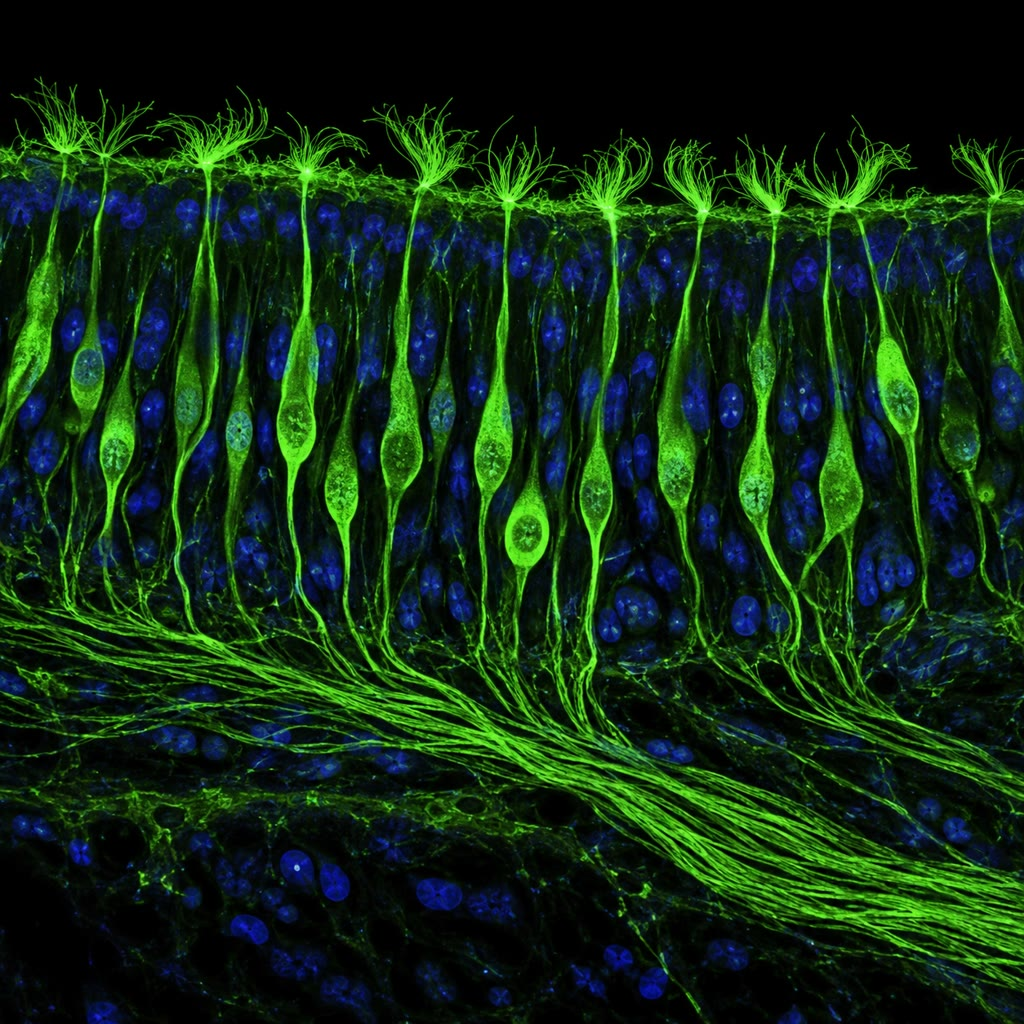
\includegraphics[width=0.40\linewidth]{images/book5/ai/b5-18-olfactory-epithelium.jpg}

{\small Het reukepitheel: zintuiglijke neuronen (groen) met
trilhaardragende dendrieten aan het oppervlak, waar geurstoffen binden,
en axonen die zich daaronder bundelen naar de bol. Elk neuron brengt
één receptorgen van de vierhonderd tot expressie.}
\end{omfigure}

\section{Tast, temperatuur, pijn en de zintuigen die ontbreken}

\begin{definition}[Lichaamsgevoel]\label{def:b3:sensory-systems:somato}
\index{mechanoreceptor}\index{Piezo-kanaal}\index{TRP-kanaal}\index{nociceptor}\index{proprioceptie}
De huid bevat verscheidene soorten \emph{mechanoreceptor}, elk een
axonuiteinde in zijn eigen kapsel: Merkel-cellen voor fijne druk en
textuur (traag aanpassend, kleine velden), lichaampjes van Meissner
voor lichte aanraking en glijden (snel aanpassend), lichaampjes van
Pacini diep in de huid voor trilling (zeer snel aanpassend, enorme
velden), Ruffini-uiteinden voor rek. De omzetter is in de meeste
daarvan \emph{Piezo2}, een reusachtig ionkanaal met een propeller van
bladen dat opengaat wanneer het membraan wordt gerekt; zonder dat
kanaal gaan de tast en het gevoel voor de stand van het lichaam
verloren, en hetzelfde kanaal in de longen en de blaas voelt hun
vulling. \emph{Temperatuur} wordt gevoeld door kanalen van de
TRP-familie die op verschillende bereiken zijn afgestemd --- TRPV1,
geopend door hitte boven \qty{43}{\celsius} en door capsaïcine, en
daarom is peper ``heet''; TRPM8, geopend door koude en door menthol ---
en \emph{pijn} door vrije zenuwuiteinden, de \emph{nociceptoren}, die
antwoorden op schadelijke hitte, druk of stoffen (protonen, ATP,
bradykinine) en wier drempels door \omterm{def:b3:innate-immunity:inflammation}{ontsteking} worden verlaagd
(\cref{ch:b3:innate-immunity}). \emph{Proprioceptie}, het gevoel voor
waar de ledematen zich bevinden, komt van de spierspoelen en
peesorganen van \cref{ch:b3:nervous-systems} en van Piezo2 in de
gewrichtskapsels. De dichtheid van de receptoren bepaalt de scherpte:
twee punten op \qty{2}{mm} afstand worden op een vingertop
onderscheiden, op de rug pas op \qty{40}{mm}.
\end{definition}

\begin{method}[Een zintuig meten]\label{met:b3:sensory-systems:psychophysics}
\index{psychofysica}\index{drempel}\index{tweepuntsonderscheid}
Om een zintuiglijk kanaal te karakteriseren: (1) bepaal de
\emph{absolute drempel} door prikkels van oplopende sterkte vele malen
aan te bieden en het waargenomen aandeel te fitten --- de sterkte die
de helft van de keren wordt waargenomen --- zoals Hecht deed;
(2) bepaal de \emph{verschildrempel} bij verscheidene sterkten en toets
de \omterm{thm:b3:sensory-systems:weber}{wet van Weber}; (3) breng de \emph{ruimtelijke scherpte} in kaart met
twee prikkels op wisselende afstand (de tweepuntsproef op de huid, een
tralie op het \omterm{def:b3:sensory-systems:retina}{netvlies}); (4) breng de \emph{tijdscherpte} in kaart met
flikkering of klikken (flikkering versmelt bij ongeveer \qty{60}{Hz} in
het daglichtzien); (5) meet in een dier aan afzonderlijke afferente
vezels terwijl dezelfde prikkels worden aangeboden en leg de neurale
drempels naast de gedragsdrempels --- de psychofysica en de fysiologie
horen overeen te stemmen, en waar zij dat niet doen is het verschil wat
het brein toevoegt.
\end{method}

\begin{remark}[Andere dieren, andere zintuigen]\label{rem:b3:sensory-systems:others}
Van elk zintuig hier bestaat een uitvoering die een dier verder heeft
gedreven, en er zijn zintuigen die de mens mist. Haaien en roggen
voelen de microvoltvelden van de hartslag van een prooi door met gelei
gevulde kanalen; elektrische vissen lezen de vervormingen van hun eigen
veld om in het donker te zien. Groefkopadders brengen warme prooi in
beeld met groeven die gevoelig zijn voor infrarood; vleermuizen en
dolfijnen echoloden, en klokken de echo's van hun eigen roep op enkele
microseconden nauwkeurig terwijl zij de frequentie van de roep
bijstellen om een mot te volgen; bijen zien ultraviolet en de
polarisatie van het hemellicht en navigeren daarop; trekvogels en
zeeschildpadden voelen het magnetische veld van de aarde langs een
mechanisme waarover nog altijd wordt getwist. De neus van een hond
heeft veertig maal zoveel receptorneuronen als de menselijke en een
derde van zijn brein om ze af te lezen; een uil hoort een muis onder de
sneeuw. De beginselen veranderen niet --- een omzetter, een \omterm{def:b3:sensory-systems:principles}{gemerkte
lijn}, een code, compressie, een kaart --- en de verscheidenheid is wat
de evolutie ermee heeft gedaan.
\end{remark}

\section{Opgaven}

\begin{exercise}[$\star$]\label{exo:b3:sensory-systems:1}
Leg uit hoe het brein weet of een reeks pulsen van het oog of van het
oor komt, gegeven dat de pulsen gelijk zijn.
\end{exercise}

\begin{exercise}[$\star$]\label{exo:b3:sensory-systems:2}
Waarom hyperpolariseert licht een fotoreceptor, en wat is de
donkerstroom?
\end{exercise}

\begin{exercise}[$\star$]\label{exo:b3:sensory-systems:3}
Fluisteren is \qty{20}{dB}, een gesprek \qty{60}{dB}, een rockconcert
\qty{110}{dB}. Bereken de sterkte van elk in W/m$^{2}$ en de verhouding
tussen het luidste en het zachtste.
\end{exercise}

\begin{exercise}[$\star$]\label{exo:b3:sensory-systems:4}
Noem de vijf smaakmodaliteiten en hun receptortypen, en leg uit waarom
een verkoudheid de ``\omterm{def:b3:sensory-systems:chemical}{smaak}'' van voedsel blokkeert.
\end{exercise}

\begin{exercise}[$\star\star$]\label{exo:b3:sensory-systems:5}
De breuk van Weber voor gewicht is $0.02$. Hoeveel net merkbare stappen
liggen er tussen een gewicht van \qty{100}{g} en \qty{10}{kg}? Gebruik
de formule van Fechner en toets dat door stappen met factor
$1.02$ te tellen.
\end{exercise}

\begin{exercise}[$\star\star$]\label{exo:b3:sensory-systems:6}
Bereken met \cref{thm:b3:sensory-systems:hecht} de waarde van
$P_{\text{see}}$ voor $a = 2$, $6$ en $12$ opgenomen fotonen bij een
drempel $n = 6$. Bij welke $a$ wordt de flits de helft van de keren
gezien? Als \qty{10}{\%} van de fotonen aan het hoornvlies wordt
opgenomen, hoeveel moet de flits er dan leveren?
\end{exercise}

\begin{exercise}[$\star\star$]\label{exo:b3:sensory-systems:7}
Het middenoor bundelt de kracht van \qty{55}{mm^2} op
\qty{3}{mm^2} met een hefboom van $1.3$. Met welke factor wordt de druk
verhoogd, en in \omterm{def:b3:sensory-systems:cochlea}{decibel}? Waarom hoort iemand met vergroeide
gehoorbeentjes (otosclerose) tientallen \omterm{def:b3:sensory-systems:cochlea}{decibel} doffer?
\end{exercise}

\begin{exercise}[$\star\star$]\label{exo:b3:sensory-systems:8}
Leg uit waarom de omzettingsstroom van een \omterm{def:b3:sensory-systems:cochlea}{haarcel} binnen microseconden
verschijnt terwijl die van een fotoreceptor tientallen milliseconden
vergt, en wat elk zintuig aan zijn ontwerp wint.
\end{exercise}

\begin{exercise}[$\star\star$]\label{exo:b3:sensory-systems:9}
Een muis heeft \num{1100} receptortypen en een mens $400$. Als een geur
ongeveer \qty{5}{\%} van de typen activeert, hoeveel patronen van
precies die omvang staan er dan voor elk ter beschikking (gebruik
$\binom{R}{k}$ met $k = 0.05R$, en de benadering van Stirling
$\ln\binom{R}{k} \approx R\,H(k/R)$ met
$H(p) = -p\ln p - (1-p)\ln(1-p)$)?
\end{exercise}

\begin{exercise}[$\star\star\star$]\label{exo:b3:sensory-systems:10}
Een \omterm{def:b3:sensory-systems:retina}{staafje} isomeriseert in het donker eens per \qty{40}{s} spontaan
een \omterm{def:b3:sensory-systems:retina}{rodopsine}. Wat is bij $500$ \omterm{def:b3:sensory-systems:retina}{staafjes} die gedurende een venster van
\qty{0.1}{s} worden gevolgd het gemiddelde aantal spontane
gebeurtenissen, en de kans dat er bij toeval zes of meer optreden? Leg
uit waarom het brein de drempel bij ongeveer zes legt en niet bij één.
\end{exercise}

\begin{exercise}[$\star\star\star$]\label{exo:b3:sensory-systems:11}
De gehoorzenuw vergrendelt haar pulsen tot \qty{4}{kHz} op de fase van
het geluid, met een spreiding van ongeveer \qty{20}{\micro s}. Geluid
loopt met \qty{340}{m/s} en de oren liggen \qty{20}{cm} uiteen. Wat is
de grootste vertraging tussen de oren, welke hoekresolutie geeft een
onderscheid van \qty{10}{\micro s} nabij het midden, en waarom dient
boven \qty{4}{kHz} de plaatscode en niet de tijdsordening?
\end{exercise}

\begin{exercise}[$\star\star\star$]\label{exo:b3:sensory-systems:12}
\omterm{def:b3:sensory-systems:principles}{Laterale remming} laat een gelijkmatig grijs vlak naast een donker vlak
aan de grens lichter lijken. Modelleer een rij receptoren die elk door
hun eigen licht $I_{i}$ worden geprikkeld en door een deel $w$ van dat
van elke buur worden geremd,
$r_{i} = I_{i} - w(I_{i-1} + I_{i+1})$, en bereken het antwoord over
een sprong van $I = 1$ naar $I = 2$ met $w = 0.2$. Wat wint en wat
verliest het \omterm{def:b3:sensory-systems:retina}{netvlies} daardoor?
\end{exercise}

\section{Vraagstuk: een kaars van ver gezien}

\begin{problem}[{Weekendvraagstuk --- de fotonen van een kaars geteld
tot in een ver oog, de waarneming van de flits berekend uit de
statistiek van Poisson en de versterker van het staafje, de decibellen
van een concert omgezet in de beweging van het trommelvlies en de
stroom van een haarcel, en de code van een neus opgesomd, eindigend bij
de afstand waarop de kaars wordt gezien, de druk op het trommelvlies en
de patronen die een neus kan vormen}]
\label{pb:b3:sensory-systems:1}
Gegevens: een kaars zendt ongeveer \qty{0.01}{W} zichtbaar licht uit,
bij \qty{550}{nm} (fotonenergie $3.6\times 10^{-19}$ J). Een aan het
donker aangepaste pupil is \qty{7}{mm} wijd; \qty{10}{\%} van de
fotonen die het oog binnenkomen wordt door \omterm{def:b3:sensory-systems:retina}{rodopsine} opgenomen; het oog
integreert over \qty{0.1}{s}; de drempel is $6$ opgenomen fotonen. Elk
opgenomen foton sluit $200$ kanalen en verlaagt de donkerstroom
gedurende \qty{0.2}{s} met \qty{1}{pA}; de donkerstroom van een \omterm{def:b3:sensory-systems:retina}{staafje}
is \qty{30}{pA}. Geluid: $I_{0} =
\qty{1e-12}{W/m^2}$; het trommelvlies heeft een oppervlak van
\qty{55}{mm^2}; een haarbundel van \qty{5}{\micro m} hoog wijkt aan de
drempel \qty{0.3}{nm} uit. Reuk: $R = 400$ receptoren; de
omzettingsstroom van een \omterm{def:b3:sensory-systems:cochlea}{haarcel} is \qty{100}{pA} bij verzadiging.

\medskip
\noindent\textbf{Deel I --- Fotonen.}
\begin{enumerate}
  \item Hoeveel fotonen per seconde zendt de kaars uit?
  \item Op afstand $d$ zijn de fotonen verspreid over een bol met
        oppervlak $4\pi d^{2}$. Hoeveel komen er per seconde de pupil
        binnen op \qty{1}{km}? En op \qty{10}{km}?
  \item Hoeveel worden er op elke afstand in één integratievenster
        opgenomen? Wordt de kaars gezien (drempel $6$)?
  \item Zoek de afstand waarop het gemiddelde opgenomen aantal in een
        venster gelijk is aan $6$. Welk deel van de vensters
        overschrijdt daar volgens de statistiek van Poisson de drempel?
  \item Wat is op de afstand van vraag 4 de kans dat een gegeven
        venster van \qty{0.1}{s} in het geheel geen foton bevat? Waarom
        lijkt een zwakke ster te flikkeren?
  \item Bij volle maan nemen dezelfde \omterm{def:b3:sensory-systems:retina}{staafjes} $10^{4}$ fotonen per
        venster uit de hemel op. Leg uit waarom de kaars op
        \qty{10}{km} dan onzichtbaar is hoewel zij dezelfde fotonen
        levert.
\end{enumerate}

\medskip
\noindent\textbf{Deel II --- De versterker van het \omterm{def:b3:sensory-systems:retina}{staafje}.}
\begin{enumerate}[resume]
  \item Eén foton sluit $200$ kanalen en verlaagt de stroom met
        \qty{1}{pA}. Welke stroom draagt één kanaal, en hoeveel
        kationen per seconde is dat ($e = \qty{1.6e-19}{C}$)?
  \item Welk deel van de donkerstroom haalt één foton weg? Hoeveel
        gelijktijdige fotonen zouden het \omterm{def:b3:sensory-systems:retina}{staafje} geheel uitschakelen
        (verzadiging)?
  \item Het antwoord duurt \qty{0.2}{s}. Hoeveel kationen belet één
        foton binnen te komen? Wat is de winst in lading per foton?
  \item In daglicht bereiken $10^{5}$ fotonen per seconde een \omterm{def:b3:sensory-systems:retina}{staafje}.
        Wat gebeurt ermee, en waarom zijn de \omterm{def:b3:sensory-systems:retina}{kegeltjes}, die minder
        aanpassen en verzadigen, de receptoren van het daglicht?
  \item \omterm{def:b3:sensory-systems:retina}{Kegeltjes} hebben ongeveer $100$ fotonen nodig om te melden.
        Verklaar met de afweging tussen gevoeligheid en snelheid waarom
        \omterm{def:b3:sensory-systems:retina}{kegeltjes} in \qty{20}{ms} antwoorden en \omterm{def:b3:sensory-systems:retina}{staafjes} in
        \qty{200}{ms}.
  \item Een \omterm{def:b3:sensory-systems:retina}{rodopsine} isomeriseert eens per \qty{40}{s} spontaan.
        Hoeveel valse fotonen per seconde brengt het \omterm{def:b3:sensory-systems:retina}{netvlies} voort
        over de $10^{8}$ \omterm{def:b3:sensory-systems:retina}{staafjes} van een oog, en waarom verblindt dat
        het donkere oog niet met ruis? (Denk aan de drempel en het
        receptieve veld.)
\end{enumerate}

\medskip
\noindent\textbf{Deel III --- \omterm{def:b3:sensory-systems:cochlea}{Decibel}.}
\begin{enumerate}[resume]
  \item Een concert van \qty{110}{dB}: sterkte in W/m$^{2}$ en het
        vermogen dat op één trommelvlies valt.
  \item Hoeveel akoestische energie ontvangt het trommelvlies tijdens
        een concert van twee uur? Vergelijk met de energie van een
        vallende regendruppel (\qty{1e-4}{J}).
  \item De gehoordrempel bij \qty{0}{dB}: vermogen op het trommelvlies
        en energie per \qty{10}{ms} --- vergelijk met de energie van
        één zichtbaar foton.
  \item De haarbundel wijkt aan de drempel \qty{0.3}{nm} uit over een
        hoogte van \qty{5}{\micro m}. Welke hoek is dat, in graden?
        Vergelijk de uitwijking met de diameter van een waterstofatoom
        (\qty{0.1}{nm}).
  \item Langdurige blootstelling boven \qty{85}{dB} beschadigt
        \omterm{def:b3:sensory-systems:cochlea}{haarcellen}, en \omterm{def:b3:sensory-systems:cochlea}{haarcellen} groeien bij zoogdieren niet aan. Twee
        uur bij \qty{110}{dB} leveren evenveel energie als hoeveel uur
        bij \qty{85}{dB}?
  \item Het bereik van het gehoor is \qty{120}{dB}. Hoeveel net
        merkbare stappen in luidheid zijn dat, als de breuk van Weber
        voor sterkte ongeveer $0.25$ is (één \omterm{def:b3:sensory-systems:cochlea}{decibel})?
\end{enumerate}

\medskip
\noindent\textbf{Deel IV --- De code van de reuk.}
\begin{enumerate}[resume]
  \item Hoeveel patronen zijn er met $400$ receptoren die elk aan of
        uit staan? Geef het antwoord als macht van tien.
  \item Als een geur gewoonlijk $20$ receptoren activeert, hoeveel
        verschillende zulke patronen zijn er dan ($\binom{400}{20}$,
        gebruik Stirling of logaritmen)?
  \item Twee geurstoffen delen $15$ van hun $20$ receptoren. Stel een
        maat voor hun afstand in de code voor en leg uit waarom zij in
        geur op elkaar lijken.
  \item Mensen onderscheiden ongeveer een biljoen geuren. Welk deel van
        de patronen van vraag 20 is dat, en wat begrenst het aantal ver
        onder de capaciteit van de code?
  \item Een muis met \num{1100} receptoren: hoeveel patronen van $20$
        meer dan een mens, als macht van tien?
  \item Een mutatie verwijdert één receptorgen. Voorspel het gevolg
        voor het reukvermogen in het algemeen en voor de waarneming van
        één geurstof die sterk aan die receptor bindt (specifieke
        anosmie).
  \item Vat samen: de afstand waarop de kaars wordt gezien (vraag~4),
        de akoestische energie op het trommelvlies aan de drempel in
        \qty{10}{ms} (vraag~15), en het aantal patronen van twintig
        receptoren dat een menselijke neus kan vormen (vraag~20).
\end{enumerate}
\end{problem}
